\section{Design}
In questa sezione esporremo il design del progetto, partendo dalle decisioni prese in ambito architetturale e proseguendo
col design di dettaglio.

\subsection{Design architetturale}
Come precedentemente illustrato nei capitoli precedenti, il progetto si propone di sviluppare un meccanismo per la creazione di sistemi multi-agente distribuiti utilizzando \textit{JaKTa}.
Il gruppo ha deciso di raggiungere questo obiettivo fornendo un'estensione del framework e del suo Domain Specific Language il più minimale possibile.
Dal punto di vista architetturale, il progetto si colloca come modulo a sé stante, come mostrato nella figura \ref{fig:architecture}:

\begin{figure}[ht!]
    \centering
    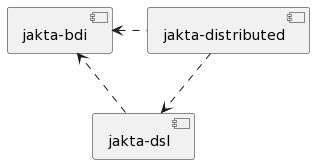
\includegraphics[width=0.8\textwidth]{figures/general-architecture.png}
    \caption{Architettura del progetto}
    \label{fig:architecture}
\end{figure}

In particolare, il modulo sviluppato è formato da tre componenti principali, come mostrato nella figura \ref{fig:detailed-architecture}:

\begin{figure}[ht!]
    \centering
    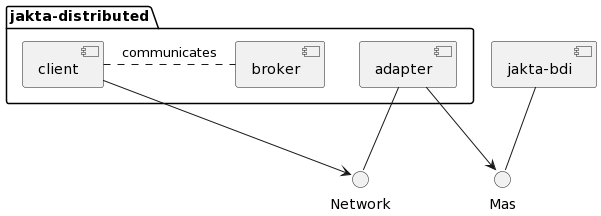
\includegraphics[width=0.8\textwidth]{figures/detailed-architecture.png}
    \caption{Architettura del modulo sviluppato}
    \label{fig:detailed-architecture}
\end{figure}

Dei moduli rappresentati in figura \ref{fig:detailed-architecture}, il modulo \textit{Adapter} è quello che definisce e contiene tutti i concetti da implementare per realizzare l'obiettivo di progetto,
mentre i moduli \textit{Client} e \textit{Broker} forniscono una prima implementazione della logica di comunicazione tra i sistemi multi-agente distribuiti.\\

Come anticipato in precedenza, il progetto presenta anche un'estensione del Domain Specific Language di JaKTa, la cui struttura è rappresentata nella figura \ref{fig:dsl-architecture}.

\begin{figure}[ht!]
    \centering
    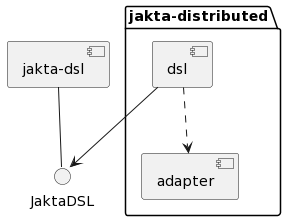
\includegraphics[width=0.8\textwidth]{figures/dsl-architecture.png}
    \caption{Architettura del Domain Specific Language}
    \label{fig:dsl-architecture}
\end{figure}

\subsection{Design di dettaglio}
La soluzione proposta consiste nell'implementazione di una versione alternativa dell'interfaccia \textit{Mas}, chiamata \textit{Dmas}, da utilizzare in contesti distribuiti.
Questa estensione dovrà comportarsi come un Mas, ma in aggiunta dovrà essere in grado di comunicare con altri Dmas attraverso la rete.

\subsubsection{Adapter}
Questo modulo si occupa di definire i concetti di:
\begin{itemize}
    \item \textbf{Dmas}: rappresenta un sistema multi-agente distribuito, cioè che può comunicare con altri sistemi Dmas attraverso la rete.
    \item \textbf{Network}: incapsula la logica di comunicazione tra Dmas attraverso la rete.
    \item \textbf{RemoteService}: rappresenta un agente remoto, cioè un agente che appartiene ad un Dmas diverso da quello corrente, ma contattabile attraverso la rete.
\end{itemize}

Le relazioni tra questi concetti sono esemplificate dal diagramma delle classi in figura \ref{fig:class-dmas}.

\begin{figure}[ht!]
    \centering
    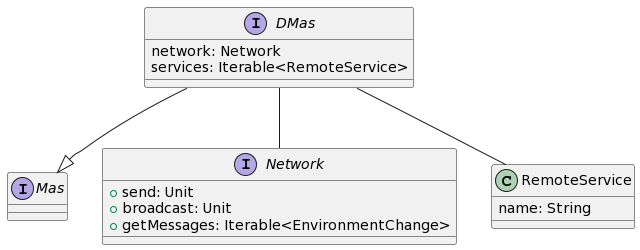
\includegraphics[width=0.8\textwidth]{figures/class-dmas.png}
    \caption{Diagramma delle classi del modulo Adapter}
    \label{fig:class-dmas}
\end{figure}

\subsubsection{Client}
Questo modulo ha lo scopo di fornire una prima implementazione del modello di comunicazione scelto per il progetto, dal punto di vista del Dmas.

\subsubsection{Broker}


\subsection{Behaviour}
Il comportamento delle varie componenti del sistema può essere descritto attraverso i seguenti passaggi:

\subsubsection{Inizializzazione del sistema}

\begin{enumerate}
    \item istanziazione di una Network;
    \item connessione da parte della Network al broker;
    \item definizione dei RemoteService di interesse;
    \item istanziazione di un Dmas;
    \item per ogni RemoteService, il Dmas si sottoscrive ai topic di interesse;
    \item esecuzione del dispatch della ExecutionStrategy scelta per il Dmas;
\end{enumerate}

Queste attività sono illustrate in figura \ref{fig:initialization}.

\begin{figure}
    \centering
    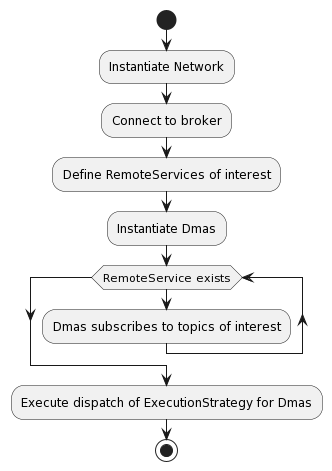
\includegraphics[width=0.8\textwidth]{figures/activity-dmas.png}
    \caption{Inizializzazione del sistema}
    \label{fig:initialization}
\end{figure}

\subsubsection{Ciclo di esecuzione del Dmas}

\begin{enumerate}
    \item il Dmas raccoglie tutti gli eventi esterni ricevuti dalla Network, ossia i messaggi pubblicati dai RemoteService a cui si è sottoscritto e le eventuali notifiche di disconnessione di un RemoteService, sotto forma di EnvironmentChange;
    \item gli eventi esterni vengono concatenati alla coda degli EncironmentChange interni del Dmas;
    \item ad uno ad uno, gli EnvironmentChange vengono processati dal Dmas. Nel caso in cui l'evento consista nell'inviare un messaggio ad un RemoteService o un broadcast, il messaggio viene inviato alla Network, che si occuperà di inoltrarlo al broker;
\end{enumerate}

Queste attività sono illustrate in figura \ref{fig:execution}.

\begin{figure}
    \centering
    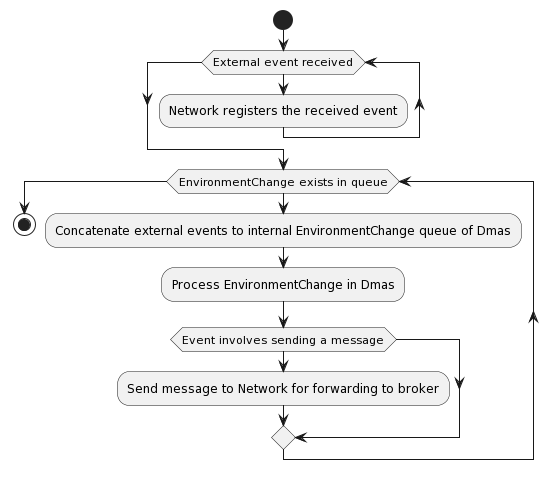
\includegraphics[width=0.8\textwidth]{figures/activity-applychanges.png}
    \caption{Ciclo di esecuzione del Dmas}
    \label{fig:execution}
\end{figure}

\subsection{Interaction}
Il modello di interazione tra i vari Dmas collegati alla rete è di tipo publish-subscribe: ogni Dmas, che assume il ruolo di client, può sottoscrivere ad uno o più topic, e può pubblicare messaggi su uno o più topic.
I messaggi pubblicati su un topic vengono ricevuti da tutti i client che si sono sottoscritti a quel topic.
Il broker, che assume il ruolo di server, si occupa di gestire la comunicazione tra i client, in particolare si occupa di:
\begin{itemize}
    \item ricevere i messaggi pubblicati dai client;
    \item inviare i messaggi ai client sottoscritti ai topic corrispondenti;
    \item gestire le connessioni e le disconnessioni dei client.
    \item gestire la sottoscrizione dei client ai vari topic.
\end{itemize}

Il comportamento di clients e broker in situazioni di broadcast e invio di messaggi con singolo destinatario è illustrato nelle figure \ref{fig:interaction-broadcast} e \ref{fig:interaction-sendmessage}.

\begin{figure}[ht!]
    \centering
    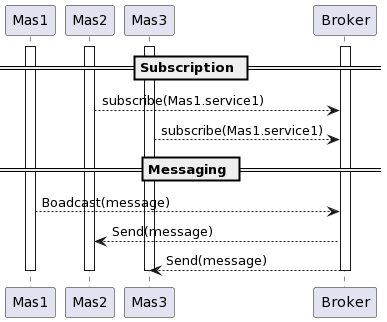
\includegraphics[width=0.8\textwidth]{figures/interaction-broadcast.png}
    \caption{Interazione tra DMas, client e broker in caso di broadcast}
    \label{fig:interaction-broadcast}
\end{figure}

\begin{figure}[ht!]
    \centering
    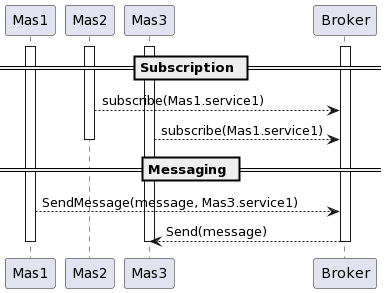
\includegraphics[width=0.8\textwidth]{figures/interaction-sendmessage.png}
    \caption{Interazione tra DMas, client e broker in caso di invio di messaggio con singolo destinatario}
    \label{fig:interaction-sendmessage}
\end{figure}
